\documentclass{beamer}
\usetheme{Warsaw}
\usepackage{graphics}
\usepackage{amsthm}
\begin{document}
\title{Robust and optimal attitude control of spacecraft with disturbances - By Yonmook Park} 

\author{Boris Polonsky}

\institute{}

\begin{frame}
\titlepage
\end{frame}

\begin{frame}
\frametitle{Content}
\begin{itemize}
	\item Introduction
	\begin{itemize}
		\item Motivation
		\item Methodology
	\end{itemize}
	\item Formulation
	\begin{itemize}
		\item Basic assumptions
		\item Modeling
		\begin{itemize}
			\item Dynamics
			\item Kinematics
		\end{itemize}
		\item Controlling
		\begin{itemize}
			\item Robust attitude control
			\item Optimal attitude control
		\end{itemize}
	\end{itemize}
	\item Simulation
	\end{itemize}
\end{frame}

\begin{frame}
\frametitle{Introduction}
\framesubtitle{Motivation}
When we design attitude control law for spacecraft, it is desirable that the law guarantees:
\begin{itemize}
	\item the robustness with respect to disturbances and,
	\item the optimality with respect to a performance index.
\end{itemize}
\end{frame}

\begin{frame}
\frametitle{Introduction}
\framesubtitle{Methodology}
To represent the attitude motion of spacecraft with respect to earth or inertia space, we could specify the transition from one frame to another with:
\begin{itemize}
	\item Euler angles
	\item Unit quaternion
\end{itemize}
\end{frame}

\begin{frame}
\frametitle{Introduction}
\framesubtitle{Methodology}
Pros and cons:
\begin{itemize}
	\item Pros of Euler angles
	\begin{itemize}
		\item Intuitive interpretation
		\item pitch, yaw, roll
	\end{itemize}
	\item Cons of both
	\begin{itemize}
		\item Singular configuration (the inherit property)
		\item Occurs at some orientations
	\end{itemize}
\end{itemize}
\end{frame}

\begin{frame}
\frametitle{Introduction}
\framesubtitle{Methodology}
\begin{itemize}
	\item Establish the model with Euler angles
	\begin{itemize}
		\item Dynamics
		\item Kinematics
	\end{itemize}
	\item Propose a control law that stabilize the system (with disturbance included)
	\item Verify the control law as the solution of the optimal game-theoretic problem. 
\end{itemize}
\end{frame}

\begin{frame}
\frametitle{Formulation}
\framesubtitle{Basic assumptions}
It is assumed that:
\begin{itemize}
	\item The disturbance has information of the system state. 
	\item It tries to maximize the performance index that the control law tries to minimize. 

\end{itemize}
The control law will be the solution of this optimal game-theoretic problem.
\end{frame}

\begin{frame}
\frametitle{Formulation}
\framesubtitle{Modeling-Dynamics}
The dynamic equation of the rotational motion of spacecraft with disturbances is given as below:
\begin{equation} \label{Dynamics}
J{\dot{\omega}(t)}=S(\omega(t))J\omega(t)+u(t)+G\xi(t)
\end{equation}
where
\begin{itemize}
	\item $\omega(t)=\begin{bmatrix}
	\omega_{1}(t)&\omega_{2}(t)&\omega_{3}(t)
	\end{bmatrix}^{T} \in \mathcal{R}^{3}$ is the angular velocity of space craft in the spacecraft body-fixed frame
	\item $u(t)=\begin{bmatrix}
	u_{1}(t)&u_{2}(t)&u_{3}(t)
	\end{bmatrix}^T \in \mathcal{R}^{3}$ is the control torque vector of spacecraft
	\item $\xi(t)=\begin{bmatrix}
	\xi_{1}(t)&\xi_{2}(t)&\xi_{3}(t)
	\end{bmatrix}^T \in \mathcal{R}^{3}$ is the disturbance vector
	\item $J \in \mathcal{R}^{3\times3}$ is the inertia matrix of spacecraft s.t $J=J^{T}>0$
	\item $G \in \mathcal{R}^{3\times3}$ is the input matrix for $\xi(t)$
\end{itemize}
\end{frame}

\begin{frame}
\frametitle{Formulation}
\framesubtitle{Modeling-Dynamics}
$S(\omega(t))$ is defined as
\begin{equation}
S(\omega(t))=\begin{bmatrix}
0&\omega_{3}(t)&-\omega_{2}(t)\\
-\omega_{3}(t)&0&\omega_{1}(t)\\
\omega_{2}(t)&-\omega_{1}(t)&0
\end{bmatrix}
\end{equation}
and has the follow property:
\begin{equation}\label{sProperty}
\omega(t)^TS(\omega(t))\equiv 0
\end{equation}
for all $\omega(t)$.
\end{frame}

\begin{frame}
\frametitle{Formulation}
\framesubtitle{Modeling-Kinematics}
The kinematic equation of the rotational motion of spacecraft represented in terms of Euler angles is shown as below:
\begin{equation} \label{Kinematics}
\dot{r}(t)=F(r(t))\omega(t)
\end{equation}
\end{frame}

\begin{frame}
\frametitle{Formulation}
\framesubtitle{Modeling-Kinematics}
where $F(r(t))$ is defined as:
\begin{equation}
F(r(t))=\begin{bmatrix}
1&\sin\phi(t)\tan\theta(t)&\cos\phi(t)\tan\theta(t)\\
0&\cos\phi(t)&-\sin\phi(t)\\
0&\sin\phi(t)\sec\theta(t)&\cos\phi(t)\sec\theta(t)\\
\end{bmatrix}
\end{equation}
\end{frame}

\begin{frame}
\frametitle{Formulation}
\framesubtitle{Modeling-Kinematics}
A singular occurs when:
$$\theta(t)=(n+\frac{1}{2})\pi$$
where $n$ is an integer. \\
\begin{itemize}
	\item It's the inherent property of all different sets of Euler angles. 
	\item For unity quaternion (a different sets of Euler angles), there are two equilibrium points that correspond to such attitudes. 
\end{itemize}
\end{frame}

\begin{frame}
\frametitle{Formulation}
\framesubtitle{Controlling-Robust attitude control}
Rayleigh-Ritz's theorem:
\begin{equation}\label{Rayleigh-Ritz's theorem}
\lambda_{min}(A)\lVert x(t)\rVert^{2}\leq x(t)^{T}Ax(t)
\end{equation}
where
\begin{itemize}
	\item $A\in \mathcal{R}^{3}$ is a Hermitian matrix
	\item $\lambda_{min}(\cdot)$ is the smallest eigenvalue of a given matrix. 
	\item $\lVert \cdot \rVert$ denotes the Euclidean norm of a vector.
\end{itemize} 
\end{frame}

\begin{frame}
\frametitle{Formulation}
\framesubtitle{Controlling-Robust attitude control}
Spectral norm of a matrix $B\in \mathcal{R}^{n\times n}$ is defined as:
\begin{equation}
\lVert B\rVert_{M}=\sqrt{\lambda_{max}(B^{T}B)}
\end{equation}
where $\lambda_{max}(\cdot)$ denotes the largest eigenvalue of a given matrix. 
\end{frame}

\begin{frame}
\frametitle{Formulation}
\framesubtitle{Controlling-Robust attitude control}
\begin{theorem}[1]
	For the attitude motions given by (\ref{Dynamics}) and (\ref{Kinematics}), let the control law be
	\begin{equation} \label{ctrlLawGen}
	u(t)=-K_{\omega}\omega(t)-F(r(t))^{T}K_{r}r(t)
	\end{equation}
	in which $K_{\omega}=K_{\omega}^{T}>0$ and $K_{r}=K_{r}^{T}>0$ are $3\times3$ Hermitian positive definite matrices. Suppose that the following conditions hold:
	\begin{equation}\label{disturbanceUpperBound}
	\lVert \xi(t)\rVert\leq\alpha\lVert\omega(t)\rVert(=\delta)
	\end{equation}
	for all $\xi(t)$ and $\omega(t)$ and
	\begin{equation}\label{feedbackGainCondition}
	\lambda_{min}(K_{\omega})>\alpha\lVert G\rVert_{M}
	\end{equation}
	 where $\alpha>0$ and $\delta>0$. Then the control law $u(t)$ of (\ref{ctrlLawGen}) is asymptotically stabilizing for the complete attitude motion of spacecraft. 
\end{theorem}
\end{frame}

\begin{frame}
\frametitle{Formulation}
\framesubtitle{Controlling-Robust attitude control}
\begin{proof}
	We choose the following Lyapunov function:
	\begin{equation}\label{Lyapunov}
	V(\omega(t),r(t))=\frac{1}{2}\omega(t)^{T}J\omega(t)+\frac{1}{2}r(t)^{T}K_{r}r(t)
	\end{equation}
	taken into account the control law in (\ref{ctrlLawGen}) and the properties of (\ref{sProperty}) and (\ref{Rayleigh-Ritz's theorem}), we obtain the time derivative of $V(\omega(t),r(t))$:
\end{proof}
\end{frame}

\begin{frame}
\frametitle{Formulation}
\framesubtitle{Controlling-Robust attitude control}
\begin{proof}
	\begin{equation}\label{timeDerivative}
	\begin{split}
	\dot{V}({\omega}(t),r(t))&=\omega(t)^{T}J{\dot{\omega}(t)}+r(t)^{T}K_{r}\dot{r}(t)\\
	&=\omega(t)^{T}\biggl[s(\omega(t))J\omega(t)-K_{\omega}\omega(t)\\
	&-F(r(t))^{T}K_{r}r(t)+G\xi(t)\biggr]\\
	&+r(t)^{T}K_{r}F(r(t))\omega(t)\\
	&=-\omega(t)^{T}K_{\omega}\omega(t)+\omega(t)^{T}G\xi(t)\\
	&\leq -\lambda_{min}(K_{\omega})\lVert\omega(t)\rVert^{2}+\lVert\omega(t)\rVert\lVert G\rVert_{M}\lVert\xi(t)\rVert
	\end{split}
	\end{equation}
\end{proof}
\end{frame}

\begin{frame}
\frametitle{Formulation}
\framesubtitle{Controlling-Robust attitude control}
\begin{proof}
	If the two conditions in (\ref{disturbanceUpperBound}) and (\ref{feedbackGainCondition}) hold, then the equation (\ref{timeDerivative}) becomes
	\begin{equation}
	\begin{split}
	\dot{V}(\omega(t),r(t))&\leq -\lambda_{min}(K_{\omega})\lVert\omega(t)\rVert^{2}+\lVert\omega(t)\rVert\lVert G\rVert_{M}\lVert\xi(t)\rVert\\
	&\leq -(\lambda_{min}(K_{\omega})-\alpha\lVert G\rVert_{M})\lVert \omega(t)\rVert^{2}\leq 0
	\end{split}
	\end{equation}
\end{proof}
\end{frame}

\begin{frame}
\frametitle{Formulation}
\framesubtitle{Controlling-Robust attitude control}
Given that 
\begin{itemize}
	\item $\dot{V}(\omega(t),r(t))$ is negative semidefinite
	\item $V(\omega(t),r(t))$ is positive definite and radically unbounded
	\item ${\mathcal {I}}$ contains no trajectory of the system except the trivial trajectory $x ( t ) = 0$ for $t\geq 0$, where ${\mathcal {I}}$ is the union of complete trajectories contained entirely in the set $\{\mathbf x : \dot{V}( \mathbf x) = 0 \}$
\end{itemize}
We can conclude that the origin is globally asymptotically stable. (LaSalle's invariance principle)
\end{frame}

\begin{frame}
\frametitle{Formulation}
\framesubtitle{Controlling-Robust attitude control}
Remark:
\begin{itemize}
	\item The control law does not require information of the inertia of spacecraft, which is convenient for us when we don't exactly now the inertia values. 
	\item Condition (\ref{disturbanceUpperBound}) shows that the disturbance is upper bounded by $\alpha\lVert\omega(t)\rVert$ and the angular velocity $\omega(t)$ is know to us. We can control the permissible level of disturbance for the control law. 
	\item Given that matrix $G$ plays the role of transmitting disturbance signal to the spacecraft, condition (\ref{feedbackGainCondition}) intuitively suggests that the "gain" with respect to state feedback(e.g. $\omega(t)$) should be grater than that of disturbance to assure that the state feedback component out-weights $\xi(t)$ in terms of their own respective effects to the system. 
\end{itemize}
\end{frame}

\begin{frame}
\frametitle{Formulation}
\framesubtitle{Controlling-Robust attitude control}
\begin{itemize}
	\item As $\alpha$ increases, $\lambda_{min}(K_{\omega})$ should increase as well in order to satisfy the condition in (\ref{feedbackGainCondition})
	\item To design a control law with large robustness margin, we should choose large values of $\alpha$ and $\lambda_{min}(K_{\omega})$
\end{itemize}
\end{frame}

\begin{frame}
\frametitle{Formulation}
\framesubtitle{Controlling-Robust attitude control}
\newtheorem{decayWithoutDisturbance}{Lemma}
\begin{decayWithoutDisturbance}
	For complete attitude motion of spacecraft described in (\ref{Dynamics}) and (\ref{Kinematics}), let the input matrix for disturbance $\xi(t)$ be $G=0_{3\times 3}$ and the feedback gain matrix be
	\begin{equation}
	K_{\omega}=\beta J
	\end{equation}
	where $\beta>0$ is a constant. Then the maximal decay rate of the closed-loop system will be $\beta$
\end{decayWithoutDisturbance}
\end{frame}

\begin{frame}
\frametitle{Formulation}
\framesubtitle{Controlling-Robust attitude control}
\begin{proof}
	By substituting $G=0_{3\times 3}$ and $K_{\omega}=\beta J$ into (\ref{timeDerivative}) we obtain
	\begin{equation}
	\begin{split}
	\dot{V}(\omega(t),r(t))&=-\omega(t)^{T}K_{\omega}\omega(t)+\omega(t)^{T}G\xi(t)\\
	&=-\omega(t)^{T}K_{\omega}\omega(t)\leq 0
	\end{split}
\end{equation}
for all $\omega(t)$
\end{proof}
\end{frame}

\begin{frame}
\frametitle{Formulation}
\framesubtitle{Controlling-Robust attitude control}
\begin{proof}
	Again, with the LaSalle's invariance principle, we can verify that:
	$\omega(t)=0$ and $\dot{\omega}(t)=0$ as $t \to \infty$
	From dynamic equation (\ref{Dynamics}) we obtain that $u(t)=-G\xi(t)=0$
	By taking into account the control law (\ref{ctrlLawGen})
	$$u(t)=-K_{\omega}\omega(t)-F(r(t))^{T}K_{r}r(t)$$ we obtain that:\\
	$r(t)=0$ as $t\to\infty$ (if $F(r(t))$ is non-singular)
\end{proof}
\end{frame}

\begin{frame}
\frametitle{Formulation}
\framesubtitle{Controlling-Robust attitude control}
\begin{proof}
	Given $K_{\omega}=\beta J$, we obtain:
	\begin{equation}
	\begin{split}
	\dot{V}(\omega(t),r(t))&=-\omega(t)^{T}K_{\omega}\omega(t)\\
	&=-\beta\omega(t)^{T}J\omega(t)-\beta r(t)^{T}K_{r}r(t)+\beta r(t)^{T}K_{r}r(t)\\
	&=-2\beta\left(\frac{1}{2}\omega(t)^{T}J\omega(t)+\frac{1}{2}r(t)^{T}K_{r}r(t)\right)\\
	&+\beta r(t)^{T}K_{r}r(t)\\
	&=-2\beta V(\omega(t),r(t))+\beta r(t)^{T}K_{r}r(t)
	\end{split}
	\end{equation}
\end{proof}
\end{frame}

\begin{frame}
\frametitle{Formulation}
\framesubtitle{Controlling-Robust attitude control}
\begin{proof}
	Hence, for all $\omega(t)$ and $r(t)$, the inequality
	\begin{equation}
		\dot{V}(\omega(t),r(t))+2\beta V(\omega(t),r(t))=\beta r(t)^{T}K_{r}r(t)\geq 0
	\end{equation}
	holds.\\
	Thus, we obtain
	\begin{equation}\label{decayRateBound}
		V(\omega(t),r(t))\geq V(\omega(t_{0}),r(t_{0}))e^{-2\beta(t-t_{0})}
	\end{equation}
	where $t_{0}$ is the initial time. (\ref{decayRateBound}) implies that the maximal decay rate of the closed loop system is $\beta$. 
\end{proof}
\end{frame}

\begin{frame}
\frametitle{Formulation}
\framesubtitle{Controlling-Optimal attitude control}
Consider the worst case problem in which:
\begin{itemize}
	\item the disturbance signal has the information of system states, and
	\item it tries to maximize the exact performance index that the control law aims to minimize
\end{itemize}
\end{frame}

\begin{frame}
\frametitle{Formulation}
\framesubtitle{Controlling-Optimal attitude control}
\begin{theorem}
	For the complete attitude motion of spacecraft given by (\ref{Dynamics}) and (\ref{Kinematics}), the control law in (\ref{ctrlLawGen}) and the disturbance given by
	\begin{equation}\label{Theorem 2 xi optimal}
	\xi(t)=W^{-1}G^{T}\omega(t)
	\end{equation}
	where $W>0$ is $3\times 3$ positive definite Hermitian matrix are optimal with respect to the performance index
	\begin{equation}\label{performanceIndex}
		\begin{split}
	\mathcal{P}=&\frac{1}{2}\int_{0}^{\infty}
	\left[x(t)^{T}Qx(t)\right.\\
	&\left.+2u(t)^{T}Nx(t)+u(t)^{T}Ru(t)-\xi(t)^{T}W\xi(t)\right]\mathrm{d}t
	\end{split}
	\end{equation}
\end{theorem}
\end{frame}

\begin{frame}
\frametitle{Formulation}
\framesubtitle{Controlling-Optimal attitude control}
\begin{theorem}
	where:\begin{itemize}
		\item $x(t)=\begin{bmatrix}
		\omega(t)^{T}&r(t)^{T}
		\end{bmatrix}^{T}\in \mathcal{R}^{6\times 1}$ is the state vector
		\item $Q\in \mathcal{R}^{6\times 6}$, $N \in \mathcal{R}^{3\times 6}$ and $R \in \mathcal{R}^{3\times 3}$ are defined by
		\begin{equation}\label{Q}
		Q=\begin{bmatrix}
		K_{\omega}-GW^{-1}G^{T}&0_{3\times 3}\\
		0_{3\times 3}&K_{r}F(r(t))K_{\omega}^{-1}F(r(t))^{T}K_{r}
		\end{bmatrix}
		\end{equation}
		\begin{equation}\label{N}
		N=
		\begin{bmatrix}
		0_{3\times 3}&K_{\omega}^{-1}F(r(t))^{T}K_{r}
		\end{bmatrix}
		\end{equation}
		\begin{equation}\label{R}
		R=K_{\omega}^{-1}
		\end{equation}
		respectively, and $K_{\omega}$ satisfies
		\begin{equation}\label{Performance Index Condition}
		K_{\omega}>GW^{-1}G^{T}
		\end{equation}
	\end{itemize}
\end{theorem}
\end{frame}

\begin{frame}
\frametitle{Formulation}
\framesubtitle{Controlling-Optimal attitude control}
\begin{proof}
	The game-theoretic Hamilton-Jacobi equation associated with the performance index $\mathcal{P}$ of (\ref{performanceIndex}) and the complete attitude motion of spacecraft described by (\ref{Dynamics}) and (\ref{Kinematics}) are given by
	\begin{equation}\label{Hamilton-Jacobi equation}
	\begin{split}
	-\frac{\partial \mathcal{P}}{\partial t}=&\min_{u(t)}\max_{\xi(t)}\biggl\{
	\frac{1}{2}x(t)^{T}Qx(t)+u(t)^{T}Nx(t)\\
	&+\frac{1}{2}u(t)^{T}Ru(t)-\frac{1}{2}\xi(t)^{T}W\xi(t)\\
	&+\frac{\partial \mathcal{P}}{\partial \omega(t)^{T}}\bigl[J^{-1}S(\omega(t))J\omega(t)+J^{-1}u(t)\\
	&+J^{-1}G\xi(t)\bigr]+\frac{\partial \mathcal{P}}{\partial r(t)^T}\bigl[F(r(t))\omega(t)\bigr]
	\biggr\}
	\end{split}
	\end{equation}
	\begin{itemize}
		\item Note: Unlike the notations in the original article, the gradient are treated as column vectors by default in the whole slide. 
	\end{itemize}
	
\end{proof}
\end{frame}

\begin{frame}
\frametitle{Formulation}
\framesubtitle{Controlling-Optimal attitude control}
\begin{proof}
	By setting the gradients of right-hand side term in (\ref{Hamilton-Jacobi equation}) with respect to $u(t)$ and $\xi(t)$ to zero vectors, we obtain the optimal control $u(t)$ and $r(t)$ shown as below:
	\begin{equation}\label{uOptimal}
	u^{*}(t)=-F(r(t))^{T}K_{r}r(t)-K_{\omega}J^{-1}\frac{\partial \mathcal{P}}{\partial \omega(t)}
	\end{equation}
	and
	\begin{equation}\label{xiOptimal}
	\xi^{*}(t)=W^{-1}G^{T}J^{-1}\frac{\partial \mathcal{P}}{\partial \omega(t)}
	\end{equation}.
\end{proof}
\end{frame}

\begin{frame}
\frametitle{Formulation}
\framesubtitle{Controlling-Optimal attitude control}
\begin{proof}
Substitute $u^{*}(t)$ of (\ref{uOptimal}) and $\xi^{*}(t)$ of (\ref{xiOptimal}) into Equation (\ref{Hamilton-Jacobi equation}), we obtain
\begin{equation}\label{Hamilton-Jacobi equation 2}
\begin{split}
-\frac{\partial \mathcal{P}}{\partial t}&=\min_{u(t)}\max_{\xi(t)}\biggl\{
\frac{1}{2}\omega(t)^{T}K_{\omega}\omega(t)-\frac{1}{2}\omega(t)^{T}GW^{-1}G^{T}\omega(t)\\
	&-\frac{\partial \mathcal{P}}{\partial \omega(t)^{T}}J^{-1}F(r(t))^{T}K_{r}r(t)\\
	&\frac{\partial \mathcal{P}}{\partial \omega(t)^{T}}J^{-1}S(\omega(t))J\omega(t)\\
	&\frac{\partial \mathcal{P}}{\partial r(t)^{T}}F(r(t))\omega(t)
	-\frac{1}{2}\frac{\partial \mathcal{P}}{\partial \omega(t)^{T}}J^{-1}K_{\omega}J^{-1}\frac{\partial \mathcal{P}}{\partial \omega(t)}\\
	&+\frac{1}{2}\frac{\partial \mathcal{P}}{\partial \omega(t)^{T}}J^{-1}GW^{-1}G^{T}J^{-1}\frac{\partial \mathcal{P}}{\partial \omega(t)}
	\biggr\}
\end{split}
\end{equation}
.
\end{proof}
\end{frame}

\begin{frame}
\frametitle{Formulation}
\framesubtitle{Controlling-Optimal attitude control}
Problems?
\begin{itemize}
	\item Given that we have set the gradients with respect to $\omega(t)$ and $r(t)$ to $\vec{0}$ and substituted the corresponding results into the Hamilton-Jacobi equation in (\ref{Hamilton-Jacobi equation}),
	\item we should omit both $\min_{u(t)}$ and $\max_{\xi(t)}$ operators on the right-hand side. 
\end{itemize}
\end{frame}

\begin{frame}
\frametitle{Formulation}
\framesubtitle{Controlling-Optimal attitude control}
\begin{proof}
	Now we consider the Lyapunov function candidate $V(\omega(t),r(t))$ of (\ref{Lyapunov}). Then $V(\omega(t),r(t))$ of (\ref{Lyapunov}) solves the equation (\ref{Hamilton-Jacobi equation 2}). \\
	Note that,
	\begin{equation}
	\frac{\partial V(\omega(t),r(t))}{\partial t}=0,\frac{\partial V}{\partial \omega(t)}=J\omega(t),\frac{\partial V}{\partial r(t)}=K_{r}r(t)
	\end{equation}
	and that $\omega(t)^{T}S(\omega(t))\equiv0$ (property of (\ref{sProperty}))
\end{proof}
\end{frame}

\begin{frame}
\frametitle{Formulation}
\framesubtitle{Controlling-Optimal attitude control}
\begin{proof}
	If the condition in (\ref{Performance Index Condition})(l.e $K_{\omega}>GW^{-1}G^{T}$) holds
	\begin{equation}
	\begin{split}
	\dot{V}({\omega}(t),r(t))&=\omega(t)^{T}J{\dot{\omega}(t)}+r(t)^{T}K_{r}\dot{r}(t)\\
	&=\omega(t)^{T}\biggl[s(\omega(t))J\omega(t)-K_{\omega}\omega(t)\\
	&-F(r(t))^{T}K_{r}r(t)+GW^{-1}G^{T}\omega(t)\biggr]\\
	&+r(t)^{T}K_{r}F(r(t))\omega(t)\\
	&=-\omega(t)^{T}(K_{\omega}-GW^{-1}G^{T})\omega(t)\leq 0
	\end{split}
	\end{equation}
	Again we make use of the property (\ref{sProperty}):$$\omega(t)^{T}s(\omega(t))\equiv 0$$
\end{proof}
\end{frame}

\begin{frame}
\frametitle{Formulation}
\framesubtitle{Controlling-Optimal attitude control}
\begin{proof}
	Just like the proof of robust attitude control in the previous section, with the LaSalle invariance principle, we obtain that $\dot{\omega}(t)=0$ and $\omega(t)=0$ as $t\to \infty$. \\
	Thus, as $t\to \infty$
	\begin{itemize}
	\item $u(t)=-G\xi(t)=-GW^{-1}G^{T}\omega(t)=0$
	\item $u(t)=-F(r(t))^{T}K_{r}r(t)-K_{\omega}\omega(t) \Rightarrow r(t)=0$
	\end{itemize}
\end{proof}
\end{frame}

\begin{frame}
\frametitle{Formulation}
\framesubtitle{Controlling-Optimal attitude control}
Remark:\\
If we set $G=0_{3\times 3}$ in (\ref{Dynamics}) and $W=0_{3\times 3}$, both the system and the performance index are immune to disturbance signal $\xi(t)$. Then we obtain the optimal control without disturbances, which is the special case of the game-theoretic problem in this sections. \\
That is to say, the game-theoretic problem is the generalization of the optimal attitude problem.
\end{frame}

\begin{frame}
\frametitle{Formulation}
\framesubtitle{Controlling-Optimal attitude control}
Remark:\\
In the performance index (\ref{performanceIndex}), the matrix $N$ defined in (\ref{N}) is to impose a cross penalty on control input and state vectors. 
By rewriting the optimal control law $u(t)$ in ($\ref{ctrlLawGen}$) as
\begin{equation}
u(t)=-R^{-1}\left\{\begin{bmatrix}
I_{3\times 3}&0_{3\times 3}
\end{bmatrix}+N\right\}\begin{bmatrix}
\omega(t)\\r(t)
\end{bmatrix}
\end{equation}
where $R$ is defined in (\ref{R}), we can see that $N$ is to adjust the feedback gain for the Euler angles.
\end{frame}

\begin{frame}
\frametitle{Formulation}
\framesubtitle{Controlling-Optimal attitude control}
Remark:\\
As shown in Equations (\ref{performanceIndex}-\ref{R}), the feedback gain matrix $K_{\omega}$ has impact on both state and control input. 
Indeed, the penalty on control input decreases as the penalty on states increases (more specifically the penalty on $\omega(t)$ I think). In this case the control law will act more aggressively in order to make the closed-loop system stable in a short period of time. And like versa.\\
Furthermore, the penalty on Euler angles can be adjust by $K_{r}$ besides $K_{\omega}$.
\end{frame}

\begin{frame}
\frametitle{Formulation}
\framesubtitle{Controlling-Optimal attitude control}
Remark:\\
In the point of view of spacecraft, both external disturbances (e.g. the solar radiation applied to spacecraft) and internal disturbance (e.g. disturbance torque from momentum wheel or thruster) makes the spacecraft rotate and/or translate at some speed. \\
Thus, the disturbance signal of (\ref{Theorem 2 xi optimal}) makes sense. \\
\end{frame}

\begin{frame}
\frametitle{Formulation}
\framesubtitle{Controlling-Optimal attitude control}
Remark:\\
If choose constant $\alpha$ s.t. 
\begin{equation} \label{Alpha for Optimal}
\alpha\geq\lVert W^{-1}G^{T}\rVert_{M}
\end{equation}
we obtain
\begin{equation}
\begin{split}
\lVert\xi(t)\rVert&=\lVert W^{-1}G^{T}\omega(t)\rVert\\
&\leq\lVert W^{-1}G^{T}\rVert_{M}\lVert\omega(t)\rVert\\
&\leq\alpha\lVert\omega(t)\rVert(=\delta)
\end{split}
\end{equation}
which satisfies the condition (\ref{disturbanceUpperBound}) in the robust attitude control theorem.
Hence, the control law in (\ref{ctrlLawGen}) is both both robust and optimal. \\
\end{frame}

\begin{frame}
\frametitle{Formulation}
\framesubtitle{Controlling-Optimal attitude control}
Question: Robustness vs Optimality
\begin{itemize}
	\item What about the "feedback gain condition" in (\ref{feedbackGainCondition})? 
	\item Given that for optimal solution, we have $K_{\omega}>GW^{-1}G^{T}$, but is it necessary that the condition for robustness $$\lambda_{min}(K_{\omega})>\alpha\lVert G\rVert_{M}$$ holds as well?
\end{itemize}
\end{frame}

\begin{frame}
\frametitle{Formulation}
\framesubtitle{Controlling-Optimal attitude control}
Not exactly: \\
We should choose $R$ in the performance index carefully (\ref{performanceIndex}) (because $R=K_{\omega}^{-1}$) to guarantee the robustness of the optimal control law.\\
$$\lambda_{min}(R^{-1})>\alpha\lVert G\rVert_{M}$$
\end{frame}

\begin{frame}
\frametitle{Formulation}
\framesubtitle{Controlling-Optimal attitude control}
Not exactly: \\
We should choose $R$ in the performance index carefully (\ref{performanceIndex}) (because $R=K_{\omega}^{-1}$) to guarantee the robustness of the optimal control law.\\
$$\lambda_{min}(R^{-1})>\alpha\lVert G\rVert_{M}$$
\end{frame}

\begin{frame}
\frametitle{Simulation}
\framesubtitle{Parameters}
Consider a specific spacecraft model:
\begin{itemize}
	\item Inertia matrix: $J=diag[5,10,15]kgm^{2}$
	\item Input matrix for disturbance signals: $G=diag[1,1.5,2]$
\end{itemize}
where "diag" implies a diagonal matrix. 
\end{frame}

\begin{frame}
\frametitle{Simulation}
\framesubtitle{Parameters}
Consider a specific spacecraft model:
\begin{itemize}
	\item Inertia matrix: $J=diag[5,10,15]kgm^{2}$
	\item Input matrix for disturbance signals: $G=diag[1,1.5,2]$
	\item $\lVert G\rVert_{M}=2$
\end{itemize}
where "diag" implies a diagonal matrix. 
\end{frame}

\begin{frame}
\frametitle{Simulation}
\framesubtitle{Parameters}
We specify following parameters
\begin{itemize}
	\item $W=I_{3\times 3}$
	\item $\alpha=2$
\end{itemize}
The select alpha satisfies the condition in (\ref{Alpha for Optimal}):
$$\alpha(=2)\geq\lVert W^{-1}G^{T}\rVert_{M}(=2)$$
\begin{itemize}
	\item $K_{\omega}=diag[5,10,15]$
	\item $K_{r}=diag[5,10,15]$
\end{itemize}
The selected $K_{\omega}$ satisfies the condition in (\ref{feedbackGainCondition})
$$\lambda_{min}(K_{\omega})(=5)>\alpha\lVert G\rVert_{M}(=4)$$
\end{frame}

\begin{frame}
\frametitle{Simulation}
\framesubtitle{Parameters}
Then we specify the feedback:
\begin{itemize}
	\item $K_{\omega}=diag[5,10,15]$
	\item $K_{r}=diag[5,10,15]$
\end{itemize}
The selected $K_{\omega}$ satisfies the condition in (\ref{feedbackGainCondition}) and (\ref{Performance Index Condition})
$$\lambda_{min}(K_{\omega})(=5)>\alpha\lVert G\rVert_{M}(=4)$$
$$K_{\omega}(=R^{-1})>GW^{-1}G^{T}$$
\end{frame}

\begin{frame}
\frametitle{Simulation}
\framesubtitle{Parameters}
And finally, we specify the initial state:
\begin{itemize}
	\item $t_{0}=0$s
	\item $\omega(t_{0})=\begin{bmatrix}
	0&0&0
	\end{bmatrix}^{T}$ rad/s
	\item $r(t_{0})=\begin{bmatrix}
	\phi(t_{0})&\theta(t_{0})&\psi(t_{0})
	\end{bmatrix}^{T}=\begin{bmatrix}
	\frac{\pi}{4}&\frac{\pi}{4}&\frac{\pi}{4}
	\end{bmatrix}^{T}$ rad
\end{itemize}
\end{frame}

\begin{frame}
\frametitle{Simulation}
Configurations for simulation:
\begin{itemize}
	\item Time interval: 0.001s
	\item Terminal time: 20s
\end{itemize}
\end{frame}

\begin{frame}
\frametitle{Simulation}
\begin{figure}[!htb]
	\center{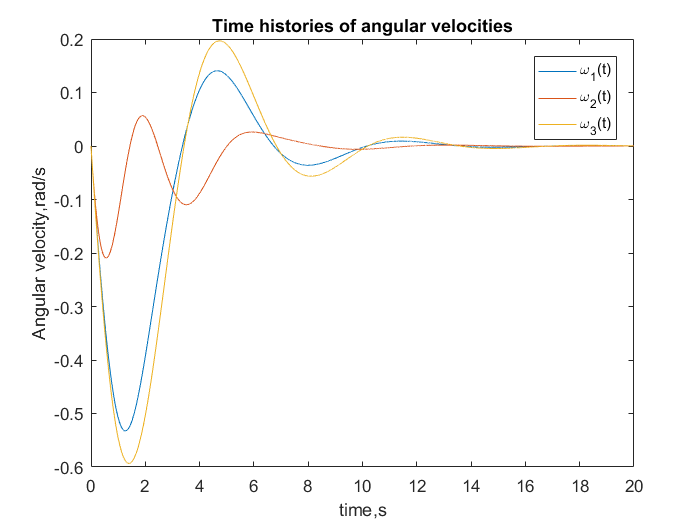
\includegraphics[width=\textwidth]  {Simulation/AngularVelocities.png}}        
\end{figure}
\end{frame}

\begin{frame}
\frametitle{Simulation}
\begin{figure}[!htb]
	\center{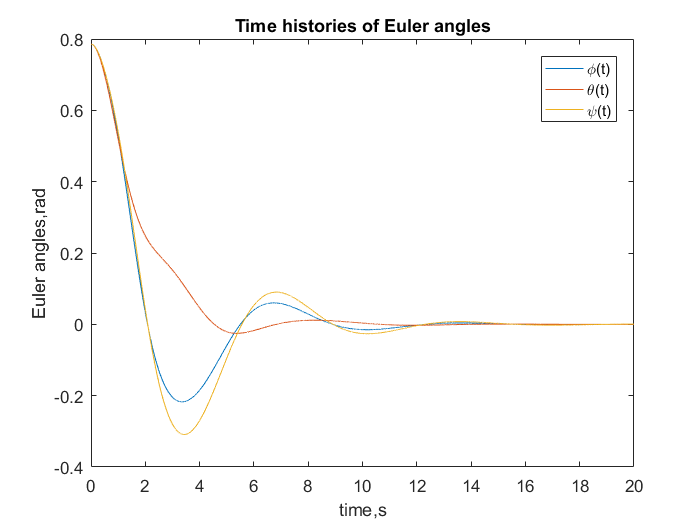
\includegraphics[width=\textwidth]  {Simulation/EulerAngles.png}}        
\end{figure}
\end{frame}

\begin{frame}
\frametitle{Simulation}
\begin{figure}[!htb]
	\center{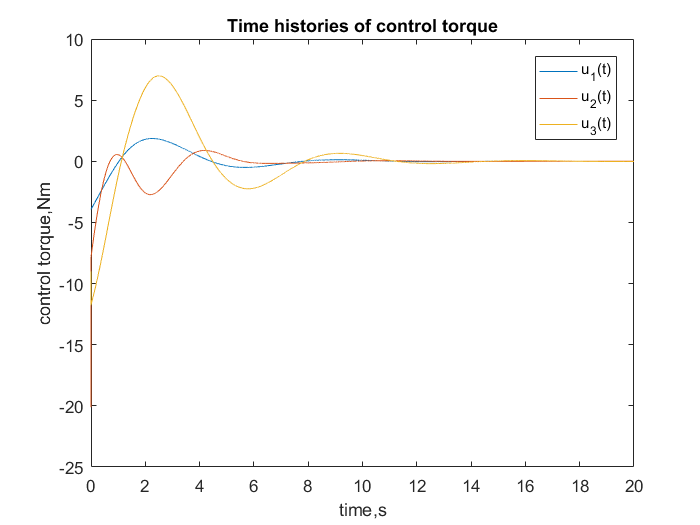
\includegraphics[width=\textwidth]  {Simulation/ControlTorque.png}}        
\end{figure}
\end{frame}

\begin{frame}
\frametitle{Simulation}
\begin{figure}[!htb]
	\center{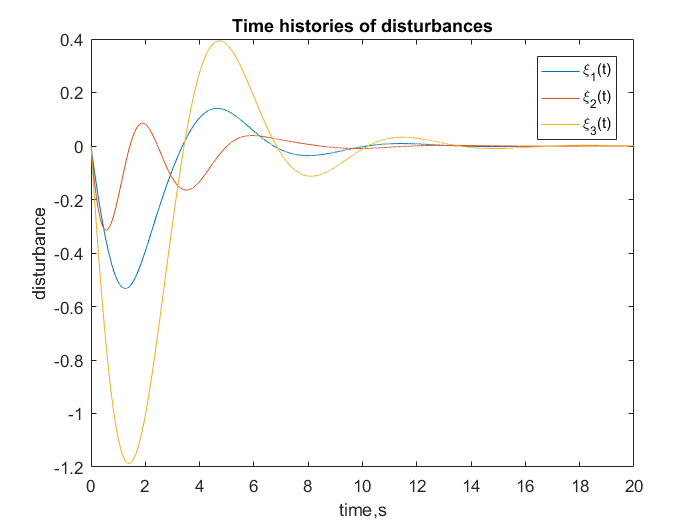
\includegraphics[width=\textwidth]  {Simulation/Disturbances.png}}        
\end{figure}
\end{frame}

\begin{frame}
\frametitle{Simulation}
\begin{figure}[!htb]
	\center{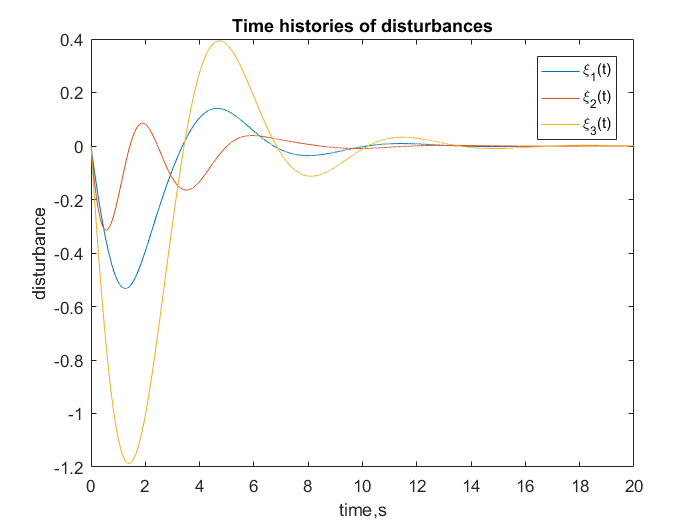
\includegraphics[width=\textwidth]  {Simulation/Disturbances.png}}        
\end{figure}
\end{frame}

\begin{frame}
\frametitle{Simulation}
\begin{figure}[!htb]
	\center{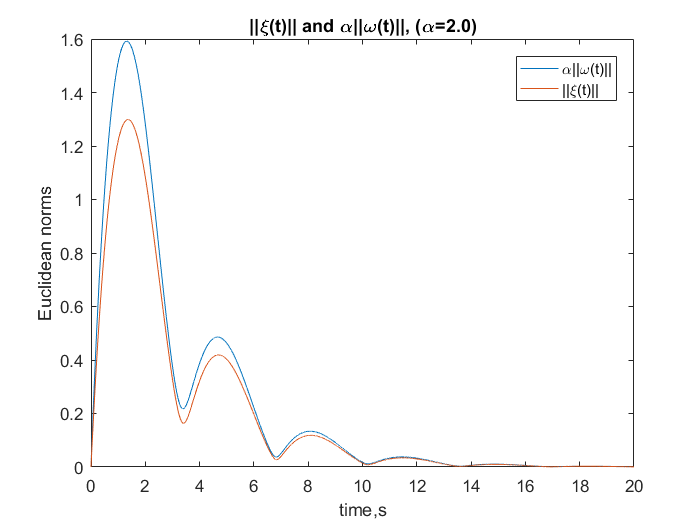
\includegraphics[width=\textwidth]  {Simulation/1stConditionOfRobustness.png}}        
\end{figure}
\end{frame}

\begin{frame}
\frametitle{Simulation}
\begin{figure}[!htb]
	\center{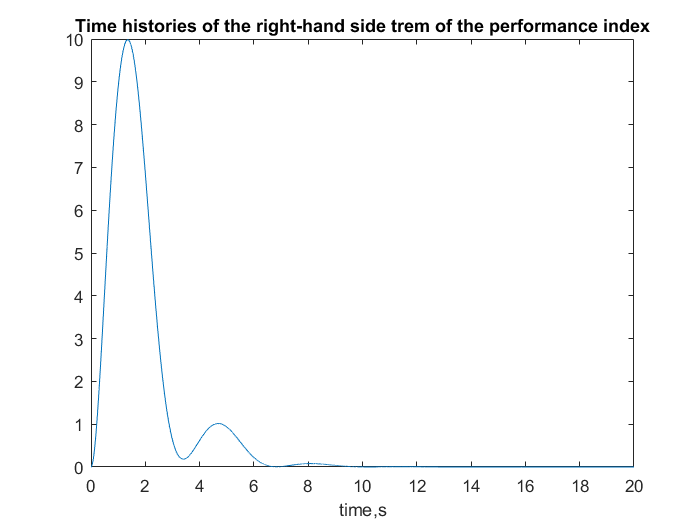
\includegraphics[width=\textwidth]  {Simulation/Performance.png}}        
\end{figure}
\end{frame}
\end{document}